\documentclass[a4paper,twoside,final]{article}
%----Eingebundene Bibliotheken-----
\usepackage[ngerman]{babel}         % Deutsches Sprachpaket
\usepackage[utf8]{inputenc}         % Eingaben codieren
\usepackage[T1]{fontenc}            % Umlaute codieren, Silbentrennung
\usepackage{amsmath, amssymb}       % Mathe
\usepackage{amsthm,amstext,amsxtra} % Symbole für Mathe
\usepackage{mathtools}              % \Aboxed Boxen in align
\usepackage{wrapfig}                % Bilder umfließen
\usepackage{svg}                    % Vektorgraphiken einbinden
\usepackage{geometry}               % Papierformat
\usepackage{tabularx}               % Tabellen
\usepackage{xcolor,colortbl}        % Farben
\usepackage{graphicx}               % Für Limes Definition wichtig
\usepackage{soul}                   % Unterstreichungen
\usepackage[section]{placeins}      % \Floatbarrier
\usepackage{wrapfig}                % Bilder umfließen
\usepackage{enumerate}              % Aufzählungen
\usepackage{footnote}               % Fußzeilen
\usepackage{booktabs}               % publication quality tables
\usepackage[hyphens]{url}           % \url{}
\usepackage{bm}                     % bold symbols \bm{r}
\usepackage{dsfont}                 % identity matrix \mathds{1}
\usepackage{enumitem}               % itemize Umgebungen customizen
\usepackage{esint}                  % Doppelintegrale
\usepackage{fancyhdr}               % schöne Kopf- und Fußzeilen
\usepackage{lmodern}
\usepackage{tikz}
\usepackage{pgfmath, pgfplots}
\usepackage[labelfont=bf]{subcaption}
\usepackage[square,numbers,sort&compress]{natbib}
\usepackage{mhchem}                 % Chemistry Package
\usepackage{physics}
\usepackage{chemfig}
\usepackage[detect-all,
            locale=DE,binary-units,
            exponent-product=\cdot
            ]{siunitx}              % \SI{12}{\gram}
%siunitx stellt für Tabellen den Spaltentyp S bereit ==> Ausrichtung an Dezimaltrennzeichen
\usepackage[position=below,
            tableposition=top,
            format=hang,
            labelfont=it,
            labelfont=bf,
            ]{caption}              % Settings für Captions
\captionsetup[wrapfigure]{name=Abb.}
\usepackage[europeanvoltages,
            europeancurrents,
            europeanresistors,
            americaninductors,
            europeanports
            ]{circuitikz}           % Schaltungen
\usepackage{chngcntr}               % vor hyperref laden!
  \counterwithin*{equation}{section}
  \counterwithin*{figure}{section}
  \counterwithin*{table}{section}

\usepackage[final,
            pdfauthor={Martin Beyer, Vanessa Huth},
            pdfsubject={Fortgeschrittenen-Praktikum},
            pdffitwindow=true,      % resize document window
            pdftitle={Fortgeschrittenen-Praktikum},
            bookmarks=true,         % lesezeichen-Liste
            bookmarksopen=true,     % Lesezeichen geöffnet
            bookmarksopenlevel=1,
            bookmarksnumbered=true,
            colorlinks=true,        % fuer Druckversion auf "false"
            linkcolor=blue,         % Table of Contents, Footnotes
            urlcolor=blue,          % fuer eingebunden URLs
            citecolor=blue,         % Equations, References
            filecolor=blue,
            pdfborder={0 0 0},      % keine Rahmen um Links: {0 0 0}
            ]{hyperref}


% Commands
\renewcommand{\sfdefault}{lmss}     % latin modern sans serif
\newcommand{\R}{\mathbb{R}}         % Reelle Zahlen
\newcommand{\N}{\mathbb{N}}         % Natürliche Zahlen
\newcommand{\C}{\mathbb{C}}         % Komplexe Zahlen
\newcommand{\de}{\mathrm{d}}      % Differential
\newcommand{\entspricht}{\mathrel{\widehat{=}}}

\DeclareSIUnit{\eV}{\text{eV}}
\DeclareSIUnit{\voltpeakpeak}{\volt{\textsubscript{pp}}}

% Dokumenteneinstellungen
\setlength{\parindent}{0px}         % remove indent in new paragraph
\setlength{\parindent}{0px}         % keine Absätze durch Leerzeilen im Code
\emergencystretch=1em % Definiert den Leerraum, der innerhalb einer Zeile zusätzlich verteilt werden darf.
\setlength{\topmargin}{-5mm} % 210mm = 8.2677165in
\newlength{\mylength}
\setlength{\mylength}{\paperwidth}
\addtolength{\mylength}{-2in} % standardmäßig wird den Seitenrändern jeweils noch 1in = 25.4mm hinzuaddiert
\setlength{\textwidth}{145mm}
\setlength{\textheight}{230mm}
\addtolength{\mylength}{-\textwidth}
\setlength{\oddsidemargin}{10mm}
\addtolength{\mylength}{-\oddsidemargin}
\setlength{\evensidemargin}{\mylength}
\setlength{\marginparwidth}{1.7cm}
\interfootnotelinepenalty=10000

% Umdefinition von \textcolor ********************************************************
\makeatletter
\renewcommand*{\@textcolor}[3]{%
	\protect\leavevmode
	\begingroup
	\color#1{#2}#3%
	\endgroup
}
\makeatother
% Damit das auch im Mathemodus anwendbar ist und dort z.B. die Leerzeichen nicht wie im Textmodus gesetzt werden.

\pgfplotsset
{compat=newest, % aktuelle Version: 1.16 [29.05.2018]
	/pgf/number format/.cd, % cd steht fuer current directory
	%  	use comma, % Komma als Dezimaltrennzeichen %%% UNCOMMENT THIS !!!
	1000 sep={} % Legt das Tausendertrennzeichen fest
}
%\usepgfplotslibrary{external} % Section 7.1.1 Using the Automatic Externalization Framework of TikZ
%\tikzexternalize[prefix=FiguresTikZ/] % activate externalization! Use subdirectory [FiguresTikZ]
\usepgfplotslibrary{fillbetween}
\usepgfplotslibrary{polar}
\usetikzlibrary{arrows.meta}
\usetikzlibrary{calc}
\usetikzlibrary{datavisualization.formats.functions}
\usetikzlibrary{intersections}
\usetikzlibrary{patterns}
\usetikzlibrary{pgfplots.colormaps}
\usetikzlibrary{plotmarks}
\usetikzlibrary{shapes.geometric}

% Generelle Festlegung des Styles fuer Blockschemata (Plaene fuer Regelkreise, etc.)
\tikzstyle{block} = [draw, fill=blue!20, rectangle, minimum height=1cm, minimum width=1cm]%, minimum width=6em]
\tikzstyle{sum} = [draw, fill=blue!20, circle, node distance=1cm]
\tikzstyle{input} = [coordinate]
\tikzstyle{output} = [coordinate]
\tikzstyle{pinstyle} = [pin edge={to-,thin,black}]

\begin{document}
\setlength{\marginparsep}{2em}
\renewcommand{\theequation}{\arabic{section}.\arabic{equation}}
\renewcommand{\thefigure}{\arabic{section}.\arabic{figure}}
\renewcommand{\thetable}{\arabic{section}.\arabic{table}}

% Anfang ********************************************************
\begin{center}
\thispagestyle{empty}
  
\includegraphics[width=0.75\textwidth]{../UniJena_BildWortMarke_black.pdf}\\[4em]
  \Large
  Ausarbeitung zum Versuch\\[2em]
  \Huge
  Radiowellen auf Leitungen\\
  und im freien Raum\\
  \vspace{2cm}
  \Large
  Martin Beyer und Vanessa Huth\\[2em]
  Abgabe: 03. Dezember 2019\\[2em]
  Betreuer: \\[5em]
  \begin{flushleft}
  	Bewertung und Ausarbeitung:\\[2em]
		Protokollführung und Form:\\[1em]
		Ergebnisse, Auswertung und Interpretation:\\[1em]
		Bemerkungen und Hinweise des Betreuers:
  \end{flushleft}
\end{center}
\clearpage

\pagestyle{fancy}
\renewcommand{\headrulewidth}{0pt}
\renewcommand{\footrulewidth}{0.5pt}
\renewcommand{\sectionmark}[1]{\markright{#1}}
\fancyhead[RO,LE]{\textbf{Radiowellen}}
\fancyhead[RE,LO]{\rightmark}
\fancyfoot[LE,RO]{\bfseries\thepage}
\fancyfoot[CO,CE]{Protokoll}
\renewcommand{\headrulewidth}{0.5pt}
\renewcommand{\footrulewidth}{0.5pt}

\setcounter{equation}{0}
\setcounter{figure}{0}

% *********************************************
% ***** KAPITEL 1 *****************************
% *********************************************
\tableofcontents
\newpage
\section{Aufgabenstellung} \label{sec:Aufgabenstellung}
\subsection{Elektromagnetische Wellen auf Leitungen}
\paragraph{Sinussignale}$~$\\
Es wird Das Verhalten von Sinussignalen auf der Leitung bei verschiedenen Kabelsorten und -anordnungen im Bereich von $1\hdots\SI{100}{\mega\hertz}$ untersucht. Es folgt eine grafische Darstellung mit Bestimmung des Verkürzungsfaktors, der Ausbreitungsgeschwindigkeit und Permittivität für die verwendeten Kabel.
\paragraph{Rechtecksignale}$~$\\
Es werden Rechtecksignale erzeugt und am \textit{Scope} mit verschiedenen Eingangswiderständen oszillographiert. Dabei werden Koaxial-Kabel unterschiedlicher Länge verwendet. Es erfolgt ebenfalls die Bestimmung der Ausbreitungsgeschwindigkeit, des Verkürzungsfaktors und der Permittivität der Anordnungen.
\paragraph{Messungen am Koaxialkabel}$~$\\
Es wird experimentell der Wellenwiderstand eines RG58 Koaxialkabels mit Rechteckimpulsen unter Verwendung verschiedener Methoden bestimmt. Zudem wird die Dispersion und das verwendete Dielektrikum des Koaxialkabels bestimmt. Für ein unbekanntest Kabelstück soll ebenfalls das Dielektrikum bestimmt werden. In einem LAN-Netzwerkkabel wird der Wellenwiderstand und der Frequenzgang bestimmt und mit dem Koaxialkabel verglichen.

\subsection{Modulation}
\paragraph{Amplitudenmodulation}$~$\\
Additive und multiplikative Amplitudenmodulation wird mithilfe von LabView simuliert. Parallel dazu wird die Modulation im Experiment realisiert und der Modulationsgrad varriert. Das amplitudenmodulierte Signal wird mithilfe eines Hüllkurvendemodulators demoduliert.
\paragraph{Frequenzmodulation}$~$\\
Die Frequenzmodulation wird mit LabView simuliert und parallel im Experiment realisert.

\subsection{Radiowellen im freien Raum}
Es sollen die Grundlagen der Dimensionierung und Berechnung von einer Halbwellendipolantenne und Viertelwellenstrahler recherchiert werden.\\
Mithilfe eines Reflektometers wird der Reflexionsfaktor eines Koaxialkabels in Abhängigkeit von der Frequenz $\SI{10}{\mega\hertz}\hdots\SI{1}{\giga\hertz}$ bestimmt. Es soll untersucht werden, welche Möglichkeiten zur messung der Ausbreitungsgeschwindigkeit in Luft realisiertbarsind.\\
Weiterhin wird ein amplitudenmoduliertes Signal über einen Halbwellendipol abgestrahlt, empfangen und demoduliert. \\
Zudem wird eine Übersicht der verwendeten Funkfrequenzen und deren Verwendungszweck erstellt. Das örtliche Frequenzspektrum und die zugehörigen Funkdienste werden bestimmt.\\
Die Ausbreitung von EM-Wellen in Wasser wird unterrsucht.
%% More to do
%%
%%


% *********************************************
% ***** KAPITEL 2 *****************************
% *********************************************
\newpage
\section{Grundlagen} \label{sec:Grundlagen}

\subsection{Elektromagnetische Wellen auf Leitungen}
Die Leitungstheorie befasst sich mit Vorgängen auf Leitungen deren Länge sich in der Größenordnung der Wellenlänge
des zu übertragenden Signals befindet, wodurch sie unter anderem in der Hochfrequenztechnik anzuwenden ist. Beispielsweise hat eine elektromagnetische Welle der Frequenz $\nu = \SI{100}{\mega\hertz}$ eine Wellenlänge von $\SI{3}{\metre}$.\\
Es gilt das Leistungsanpassungsgesetz mit $Z_Q$ als Quellwiderstand und $Z_A$, dem Abschlusswiderstand. Bei $Z_Q = Z_A$ entsteht eine Leistungsanpassung, d.\,h. maximale Leistung wird übertragen.\\
Im Hochfrequenzbereich muss eine weitere Größe, der \textit{Wellenwiderstand} $Z_L$ der Leitung berücksichtigt werden. Hierbei wird gefordert, dass $Z_L = Z_A$ idealerweise gelten muss, um stehende Wellen zu vermeiden.
\begin{figure}[htp]
    \centering
    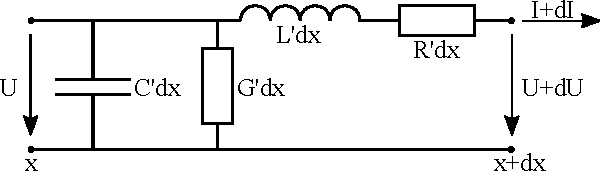
\includegraphics[width=0.8\textwidth]{Schaltungen/Ersatzschaltbild.pdf}
    \caption{Ersatzschaltbild eines homogenen Leitungsstücks von $x$ bist $x+\de x$.}
    \label{fig:Ersatzschaltbild}
\end{figure}\\

\subsection{Modulation}
Als Modulation wird das Aufprägen einer Information auf eine Trägerschwingung bezeichnet. Dabei wird das zu übertragene Nutzsignal in einen definierten höheren Frequenzbereich verschoben. Dies wird benötigt, weil der direkte Übertragungsweg des Signals durch ein Medium wie z.\,B. Schall häufig nicht über lange Strecken möglich ist. Im Allgemeinen erfolgt die Signalübertragung über einen Kanal wie Luft oder Kabel. Im Kanal tritt eine frequenzabhängige Dämpfung auf, weshalb das Signal auf eine Frequenz innerhalb eines dämpfungsarmen Frequenzfensters moduliert wird. Für das Nutzsignal und den Träger lassen sich folgende Formeln aufstellen.
\begin{align}
    U_\text{Nutz}(t) &= U_\text{N}\cdot\cos(\omega_\text{N}t) & \text{Spannung Nutzfrequenz}\\
    U_\text{Träger}(t) &= U_\text{T}\cdot\cos(\omega_\text{T}t) & \text{Spannung Trägerfrequenz}
\end{align}
Der Träger wird benötigt, um die Information des Nutzsignals durch spätere Demodulation wieder zu erhalten.\\
Die Mischung zweier Signale wird technisch auf gleiche Weise realisiert wie die Modulation. Bei der Mischung wird nur eine der entstehenden Frequenzen weiter benutzt, während bei der Modulation mehrere Mischprodukte weiter verwendet werden.
\subsubsection{Amplitudenmodulation}
Bei der Amplitudenmodulation wird das Signal in der Amplitude der Trägerschwingung kodiert. Die Amplitude des modulierten Signals ändert sich mit der Frequenz des Nutzsignals, während die Schwingungsfrequenz durch den Träger vorgegeben wird. Es lassen sich zwei verschiedene Verfahren unterscheiden.
\paragraph{Additive Amplitudenmodulation}
Hierbei handelt es sich um die am einfachsten realisierbare Variante. Die zu modulierenden Signale werden überlagert und anschließend an einer Kennlinie (Diode oder Transistor) mit exponentiellen Verlauf verzerrt. Dabei entstehen neue Frequenzkomponenten.
\begin{align}
  U_\text{AM}(t) = U_\text{T}\cos(\omega_\text{T}t) + U_\text{N}\cos(\omega_\text{N}t)\cdot\cos(\omega_\text{T}t)
\end{align}
Neben der Trägerfrequenz $\omega_\text{T}$ entstehen im amplitudenmodulierten Signal zwei weitere Frequenzen. Diese Schwebungsfrequenzen $\omega_\text{T} \pm \omega_\text{N}$ werden als Seitenbänder bezeichnet.
\begin{align}
  U_\text{oberes Seitenband}\cos(\omega_\text{T} + \omega_\text{N})\\
  U_\text{unteres Seitenband}\cos(\omega_\text{T} - \omega_\text{N})
\end{align}
Üblicherweise wird die Trägerfrequenz $\omega_\text{T}$ so gewählt, dass sie viel größer als die Signalfrequenz ist, $\omega_\text{S} \ll \omega_\text{T}$, weshalb alle auftretenden Frequenzen im Größenbereich der Trägerfrequenz liegen.\\
Eine weitere charakteristische Größe stellt der Modulationsgrad $M$ dar. Dieser ist definiert als Verhältnis der Hüllkurvenamplitude zur Trägeramplitude und berechnet sich folgendermaßen
\begin{align}
  M = \frac{U_N}{U_T} = \frac{\text{max}-\text{min}}{\text{max}+\text{min}},
\end{align}
wobei die beiden Größen in Abbildung~\ref{fig:Amplitudenmodulation} eingezeichnet sind.
\begin{figure}[htp]
    \centering
        \begin{center}
	\newcommand\maxt{2} % in [s]
	\newcommand\fTraeger{20} % in [Hz]
	\newcommand\fSignal{1.5} % in [Hz]
	\newcommand\Modulationstiefe{50} % in Prozent

	\begin{tikzpicture}[trim axis left, trim axis right]
  	\begin{axis}[
    	clip=false,
    	width=0.9\textwidth, height=0.3\textwidth,
    	xlabel={$t$ [\si{\second}]},
    	ylabel={Amplitude [\si{\volt}]},
    	xmin=0, xmax=\maxt,
    	xtick distance=0.5,
    	minor x tick num=4,
    	ytick distance=1,
    	minor y tick num=4,
    	legend style={cells={anchor=west}, legend pos=outer north east,},
    	]
      \addplot [domain=0:{\maxt}, samples=500, smooth, mark=none, thick, color=blue, solid] {cos(deg(2*pi*\fTraeger*x))*(1 + (\Modulationstiefe/100)*(cos(deg(2*pi*(\fSignal)*x))))};
      \addplot [domain=0:{\maxt}, samples=100, smooth, mark=none, thick, color=black, densely dotted, forget plot] {+1*(\Modulationstiefe/100)*cos(deg(2*pi*\fSignal*x)) + 1};
      \addplot [domain=0:{\maxt}, samples=100, smooth, mark=none, thick, color=black, densely dotted, forget plot] {-1*(\Modulationstiefe/100)*cos(deg(2*pi*\fSignal*x)) - 1};
    	\draw [thick, black, stealth-] ({0.5/\fSignal},{+1-(\Modulationstiefe/100)}) -- ({0.5/\fSignal},{+1-(\Modulationstiefe/100) + 0.4});
    	\draw [thick, black, stealth-] ({0.5/\fSignal},{-1+(\Modulationstiefe/100)}) -- ({0.5/\fSignal},{-1+(\Modulationstiefe/100) - 0.4}) node[below,fill=gray!50!white,rectangle,rounded corners=3pt]{min};
    	\draw [thick, black, stealth-] ({1/\fSignal},{+1+(\Modulationstiefe/100)}) -- ({1/\fSignal},{0});
    	\draw [thick, black, stealth-] ({1/\fSignal},{-1-(\Modulationstiefe/100)}) -- ({1/\fSignal},{0});
    	\path ({1/\fSignal},{+1+(\Modulationstiefe/100)}) -- node[fill=gray!50!white,rectangle,rounded corners=3pt]{max} ({1/\fSignal},{-1-(\Modulationstiefe/100)});
  	\end{axis}
	\end{tikzpicture}
\end{center}

    \caption{Amplitudenmodulation eines Signals $f_\text{N} = \SI{1.5}{\hertz}$ mit der Trägerfrequenz $f_\text{T} = \SI{20}{\hertz}$ mit Modulationstiefe $M = \SI{50}{\percent}$ (eigene Abbildung).}
    \label{fig:Amplitudenmodulation}
\end{figure}\\
Bei einem Modulationsgrad von $\SI{100}{\percent}$ fällt die Amplitude des modulierten Signals auf $\SI{0}{\volt}$ ab.
\paragraph{Multiplikative Amplitudenmodulation}
Diese Modulationsvariante wird in der Praxis häufiger eingesetzt und kann mit Diodenringmodulatoren realisiert werden. Dabei werden die beiden Schwingungen direkt miteinander multipliziert
\begin{align}
    U_\text{AM} = U_\text{N} \cos(\omega_\text{N}t)\cdot U_\text{T} \cos(\omega_\text{T}t).
\end{align}
Der Unterschied zur additiven Variante besteht darin, dass die Trägerfrequenz nicht mit erzeugt wird und unerwünschte Nebenfrequenzen unterdrückt werden. Das Minimum im Zeitsignal zeigt einen Phasensprung.

\subsection{Frequenzmodulation}
Bei der Frequenzmodulation wird die Amplitude des modulierten Signals konstante gehalten und durch das Trägersignal charakterisiert. Die Information des Nutzsignals

% \begin{table}[ht]
% 	\centering
% 	\caption{}
% 	\label{tab:Achsensysteme}
% 	\begin{tabular}{l l l l}
% 		\toprule
% 	 	\midrule
% 	\end{tabular}
% \end{table}\\

\subsection{Demodulation}
\begin{figure}[htp]
    \centering
    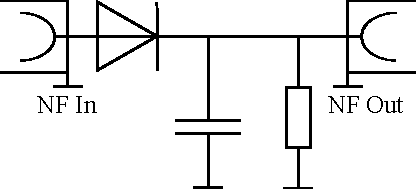
\includegraphics[width=0.5\textwidth]{Schaltungen/Demodulator.pdf}
    \caption{}
    \label{fig:Demodulator}
\end{figure}
% *********************************************
% ***** KAPITEL 3 *****************************
% *********************************************
\section{Versuchsdurchführung} \label{sec:Versuchsdurchführung}
\subsection{Elektromagnetische Wellen auf Leitungen}
\subsubsection{Verhalten von Sinussignalen auf verschiedenen Leitungen mit verschiedenen Anpassungen}
Die Frequenzgänge im Bereich \SI{1}{\mega\hertz} bis \SI{100}{\kilo\hertz} verschiedener Kabelanorndungen werden gemessen und graphisch dargestellt. Dazu wird ein HF Generator mit Ausgang ca. \SI{50}{\ohm} und nageschaltetem Teiler 10:1 mit Hilfe der jeweiligen Kabelart mit einem Scope verbunden, an welchem jeweils der Eingangswiderstand zwischen \SI{50}{\ohm}  und \SI{1}{\mega\ohm} variiert wird. An diesem wird auch die jeweilige zur Frequenz gehörenden Spannung abgelesen.  Dabei werden
\begin{itemize}
  \item Laborkabel (ca. \SI{2}{\meter} Länge)
  \begin{itemize}
    \item Scope Eingangwiderstand \SI{1}{\mega\ohm}
    \item Scope Eingangswiderstand \SI{50}{\ohm}
  \end{itemize}
  \item{Koaxialkabel (ca. \SI{2}{\meter} Länge)}
  \begin{itemize}
    \item Skope Eingangswiderstand \SI{1}{\mega\ohm}
    \item Skope Eingangwiderstand \SI{50}{\ohm}
  \end{itemize}
  \item Koaxialkabel mit über T-Stück zusätzlich angeschlossenem Stichkabel (Länge: \SI{2,48}{\meter}) bei einem Skope Eingangwiderstand von \SI{50}{\ohm}
  \begin{itemize}
    \item Abschluss des Stichkabels: offen
    \item Abschluss des Stichkabels: Kurzschluss (realisiert durch Kurzschlussstecker)
    \item Abschluss des Stichkabels: Wellenwiderstand (realisiert durch \SI{50}{\ohm}- Stecker)
  \end{itemize}
  vermessen.
\end{itemize}

Anschließend werden Verkürzungsfaktor, Ausbreitungsgeschwindigkeit und Permitivität für das Koaxialkabel mit dem vorhergehenden Messaufbau bestimmt.

\subsubsection{Verhalten von Rechtecksignalen auf der Leitung bei verschiedenen Anpassungen}
Mit dem Funktionsgenerator Agilent 33220A wird ein Rechtecksignal (\SI{50}{\nano\second}, \SI{100}{\kilo\hertz} erzeugt. Dieser ist über ein ca. \SI{2}{\meter} langes Koaxialkabel mit dem Scope verbunden, auf welchem das Signal beobachtet wird. Dabei ist dessen Eingangswiderstand einmal  \SI{50}{\ohm} und einmal \SI{1}{\mega\ohm}.
 \\
Anschließend wird ein \SI{25}{\meter} langes Koaxialkabel mit einem T-Stück als Stichkabel an das den Frequenzgenerator und Scope verbindende Kabel angeschlossen. Der Scope hat einen Eingangwiderstand von \SI{50}{\ohm}- Hier werden die Impulsformen am Anfang des Kabels bei folgenden Abschlusswiderständen am Ende des Kabels beobachtet:
\begin{itemize}
  \item $Z_A = \infty$ (offenes Leitungsende)
  \item $Z_A = 0$ (Kurzschlussstecker)
  \item $Z_A = Z_L$ (Stecker mit Wellenwiderstand \SI{50}{\ohm})

\end{itemize}

Anschließend wird für $Z_A=Z_L$ und $Z_A = \infty$ das Signal zusätzlich am Ende des Stickkabels beobachtet. Dazu wird das Ende des Stichkabels an den 2. Eingang des Scopes angeschlossen und der Eingangswiderstand dieses Eingangs einmal auf \SI{50}{\ohm} (entspricht $Z_A = Z_L$) und einmal auf \SI{1}{\mega\ohm (entspricht $Z_A = \infty$) eingestellt. \\

Außerdem wird der gleiche Rechteckpuls mit Laborkabeln übertragen. Auch hierbei wird der Eingangswiederstand einmal auf \SI{50}{\ohm} und einmal auf \SI{1}{\mega\ohm} eingestellt. \\

Die Ausbreitungsgeschwindigkeit, der Verkürzungfaktor und die Permitivität werden bestimmt, indem ein \SI{25}{\meter} langes als Stichkabel auf das den Frequenzgenerator und den Scope verbindende Kabel angebracht und ein Rechtecksignal durch die Leitung geschickt wird. Aus der Verschiebung zweier Flanken errechnet sich die Ausbreitungsgeschwindigkeit und daraus anschließend der Verkürzungsfaktor und die Permitivität. Alternativ werden alle drei Größen auch bestimmt, indem das Stichkabel mit dem Scope im zweiten Eingang mit Eingangwiderstand \SI{50}{\ohm} verbunden wird und die Verschiebung des durchlaufenden mit dem am Ende des Stichkabels ankommenden Pulses für Berechnungen genutzt wird.


\subsection{experimentelle Bestimmung des Wellenwiderstandes eines RG58 Koaxialkabels mit Rechteckimpulsen}\label{subsec:BestimmungZL}
Frequenzgenerator und Scope werden über ein kurzer Koaxialkabel miteinander verbunden. Ein \SI{50}{\meter}} langes Koaxialkabel wird als Stichkabel über ein T-Stück angeschlossen. Das Ende dieses Stichkabels wird mit einem veränderbaren Widerstand (Potentiometer) abgeschlossen. Am Scope werden die Reflexionen der Impulse am Anfang der Leitung in Abhängigkeit vom Widerstand beobachtet und diejenige EInstellung von R bestimmt, sodass die Reflexionen minimal sind. Dieser eingestellte Widerstand wird mit Hilfe eines Multimeters vermessen.

\subsection{Bestimmung des Wellenwiderstandes eines RG58 Koaxialkabels durch L und C Messung}
Für diese Messung wird eine LC-Messbrücke verwendet. Für die Messung der Kapazität wird das Leitungsende offen gelassen, wird die Induktivität gemessen, verwendet man einen Kurzschlussstecker als Abschlusswiderstand des Kabels.

% *********************************************
% ***** KAPITEL 4 *****************************
% *********************************************
\newpage
\section{Ergebnisse und Diskussion}
\subsection{Elektromagnetische Wellen auf Leitungen}
\subsubsection{Verhalten von Sinussignalen auf verschiedenen Leitungen mit verschiedenen Anpassungen}
Die im Bereich \SI{1}{\mega\hertz} bis \SI{100}{\kilo\hertz} gemessenen Frequenzgänge verschiedener Kabelanorndungen sind im Folgenden graphisch dargestellt.
\paragraph{Laborkabel (Länge ca. \SI{2}{\meter})}


Während der Messung mit den Laborkabeln fällt auf, dass sich durch kleine Veränderungen der Anordnung der Kabel bzw. Bewegung der Kabel wie zum Beispiel durch Wackeln der Wert der angezeigten Spannung bei gleicher Frequenz ändert. Eine Kabelbewegung führt also zu einem anderen Frequenzgang bzw. Spannungsverlauf. Trotz Verwendung des gleichen Kabels ist es nicht möglich, einen identischen Frequenzgang bei einer späteren Messung zu erhalten.
Im Allgemeinen weisen die Kabel sowohl bei \SI{50}{\ohm}, als auch bei \SI{1}{\mega\ohm} Eingangwiderstand des Scopes einen chaotischen Frequenzgang auf (bei \SI{1}{\mega\ohm} wurden nur globale Maxima und Minima vermessen, aber auch zwischen diesen Peaks wurden immer wieder lokale Minima und Maxima festgestellt). Bei \SI{1}{\mega\ohm} kommt es dazu, dass die Spannung bei bestimmten Frequenzen höher wird, als die, die ursprünglich herein gegeben wurde. Das Kabel wirkt hierbei als Transformator.
Auch bei Verwendung eines \SI{50}{\ohm} Eingangwiderstand des Scopes schwankt die Spannung bei Erhöhung der Frequenz merklich hin und her. Innerhalb kleiner Frequenzbereiche zeigen sich immer wieder lokale Minima und Maxima.\\
Wegen der bereits erklärten Abhängigkeit eines Spannungswertes bei gleicher Frequenz von der Anordnung der Kabel sowie des chaotischen Verlaufs auch bei \SI{50}{\ohm} des sind die Laborkabel als ungeeignet für Messungen in der Hochfrequenztechnik einzustufen.

\paragraph{Koaxialkabel (Länge ca. \SI{2}{\meter})}
Auch bei den Koaxialkabeln wird bei einem Eingangswiderstand des Scopes von \SI{1}{\mega\ohm} bei Frequenzen von ungefähr \SI{20}{\mega\hertz} und \SI{70}{\mega\hertz} Maxima festgestellt, an denen Spannungen gemessen werden, die über der Spannung liegt, die eingegeben wurde. Diese Maxima treten periodisch auf.\\
Bei einem Eingangwiderstand des Scopes von \SI{1}{\mega\ohm} liegt eine falsche Anpassung vor, welche zu Reflexion und zu stehenden Wellen führt. In den genannten Fällen kommt es so zu einer Spannungsverstärkung. Diese Eigenschaft eröffnet die Möglichkeit der Verwendung der Koaxialkabel bei diesem Frequenzen als Transformator und bietet damit eine Alternative zum Transformieren mit einem Schwingkreis.\\
Ebenso periodisch treten auch Minima auf. Hier kommt es aufgrund der Reflexionen zu Auslöschungen und damit zu niedrigeren gemessenen Spannungen. Diese eignen sich in der Praxis besser zum Auswerten. Ein Spannungsmaxima ist nicht so gut messbar, da das Messgerät in diesem Fall sehr hochohmig sein müsste. Dies ist praktisch schwer zu realisieren, weshalb es zu einer Verfälschung der Spannung bei Messung von Maxima kommt.

\paragraph{zu Koaxialkabel zustätzlich über T-Stück angeschlossenes Koaxialkabel(sogenanntes Stichkabel)(Länge \SI{2,48}{\meter}), Eingangwiderstand des Scopes \SI{50}{\ohm}}
Bei der Analyse der Frequenzgänge bei Verwendung eines Stickkabels jeweils mit offenem Ende, Kurzschlusstecker oder \SI{50}{\ohm} - Steckers fällt auf, dass in der Nähe der Frequenzen, wo die Spannung bei offenem Ende des Stickkabels, und damit nährungsweise unendlichem Abschlusswiderstand $Z_A$, ein Maximum zeigt, bei Verwendung eines Kurzschlussteckers, und damit ungefähr Abschlusswiderstand \SI{0}{\ohm}, am Ende des Stickkabels ein Maximum aufweist. \\

Zunächst wird der Fall des unendlichen Abschlusswiderstands betrachtet. Für diesen Fall muss sich am Ende des Kabels ein Spannungsmaxima befinden. Am Anfang des Kabels ist, als Bedingung für ein Minima, die Spannung nährungsweise auf 0 abgefallen. Da die Spannung sich über die Länge des Kabels sinusförmig verhält, ergibt sich, dass diese Bedingung bei
\begin{align}
  L_{\text{Stichkabel}} = \frac{\lambda_{L}}{4} \; \text{und} \; L_{\text{Stickkabel}} = \frac{3\cdot \lambda_{L}}{4}
\end{align}
bzw. allgemein bei
\begin{align}
L = \frac{(2n+1)\cdot \lambda_{L}}{4\cdot f}
\end{align}
erfüllt ist, was demnach die Bedingung für ein \textbf{Minima bei $Z_A = \infty$} darstellt. \\
Soll nun ein Maxima bei $Z_A = \infty$ beschrieben werden, ist folgende Überlegung anzustellen: Auch hier muss wegen $Z_A=\infty$ am Ende des Kabels ein Spannungsmaxima auftreten. Am Anfang des Kabels, als Bedigung für ein Maxima, tritt ebenfalls ein Spannungsmaxima auf. Bei Annahme eines sinusförmigen Verhaltens des Spannungsverlaufs über die Länge des Kabels, ergibt sich, dass diese Bedingung bei

\begin{align}
L_{\text{Stichkabel}} = \frac{\lambda_{L}}{2} \; \text{und} \; L_{\text{Stichkabel}} = \lambda_{L}
\end{align}

bzw. allgemein bei

\begin{align}
L = \frac{n \cdot \lambda_{L}}{2} \;
\end{align}

erfüllt ist, was demnach die Bedingung für ein \textbf{Maxima bei $Z_A = \infty$} darstellt. \\

Bei einem Abschlusswiderstand von $Z_A = 0$ wird am Ende der Leitung die Spannung nährungsweise auf 0 abgefallen sein. Wird hierbei ein Minima gefordert, muss am Anfang des Kabels die Spannung ebenfalls auf 0 abgefallen sein. Diese Bedingung ist bei Annahme eines sinusförmigen Verlaufs erfüllt, wenn gilt

\begin{align}
L_{\text{Stichkabel}} = \frac{\lambda_{L}}{2} \; \text{und} \; L_{\text{Stichkabel}} = \lambda_{L}
\end{align}

bzw. allgemein

\begin{align}
L = \frac{n \cdot \lambda_{L}}{2} \;
\end{align}
Dies entspricht also der Bedingung für ein \textbf{Minima bei $Z_A = 0$}.
Für ein Maxima, wird die Bedingung gestellt, dass die Spannung am Anfang des Kabels ein Maxima erreichen soll. Bei Annahme, dass die Spannung am Ende des Kabels nährungsweise 0 ist (da $Z_A = 0$) und eines sinusförmigen Verlaufs der Spannung entlang des Kabels, finden sich hier die Bedingungen
\begin{align}
  L_{\text{Stichkabel}} = \frac{\lambda_{L}}{4} \; \text{und} \; L_{\text{Stickkabel}} = \frac{3\cdot \lambda_{L}}{4}
\end{align}
bzw. allgemein bei
\begin{align}
L = \frac{(2n+1)\cdot \lambda_{L}}{4\cdot f}
\end{align}
Dies entspricht also der Bedingung für ein \textbf{Maxima bei $Z_A = 0$}.

Weiterhin wird an Hand der Messdaten festgestellt, dass obwohl mit einem \{50}{\ohm}-Stecker am Ende des Stichkabels die Widerstandsanpassung erreicht wird, keine konstante Spannung über alle Frequenzen beobachtet wird. Dies kann an leichten Abweichung des Steckers von \SI{50}{\ohm} und des Kabels von \SI{50}{\ohm} Wellenwiderstand liegen. So treten trotz der scheinbaren Anpassung leichte Reflexionen auf. \\
Es wird festgehalten, dass mit einem Stichkabel nach obigem Prinzip bewusst Frequenzen gefiltert werden können. Für $Z_{L, Kabel} = Z_A$ wird der frequenzunabhängigste Frequenzgang erreicht.\\

Zur \textbf{Bestimmung des Verkürzungsfaktor} wird das erste Minimum der Spannung bei Verwendung des Stichkabels mit offenem Ende betrachtet. Dieses wird bei \SI{20}{\kilo\hertz} bestimmt. Aufgrund vorheriger Überlegungen entspricht dies genau $\frac{\lambda_{L}}{4}$. Der Verkürzungsfaktor wird bestimmt durch
\begin{align}
K = \frac{\lambda_{L}}{\lambda_0}
\end{align}
Für den konkreten Fall lässt sich nutzen:
\begin{align}\label{equ:K}
K = \frac{\frac{\lambda_L}{4}}{\frac{\lambda_0}{4}} = \frac{\SI{2,48}{\meter}}{\frac{c}{4\cdot f}} = \frac{\SI{2,48}{\meter}\cdot 4 \cdot f}{c} = 0,661
\end{align}
Über die Relation
\begin{align}
K = \frac{1}{\sqrt{\epsilon_R}}
\end{align}
lässt sich die \textbf{Permitivität} auf
\begin{align}
\epsilon_R = \frac{1}{K^2} = 2,286
\end{align}
Die \textbf{Ausbreitungsgeschwindigkeit} erhält man dann durch
\begin{align}
c = \frac{c_0}{\sqrt(\epsilon_R)} = c_0 \cdot K = \SI{198300000}{\meter\per\second\squared}
\end{align}

 Mithilfe dieser Werte wird es möglich, eine \textbf{rechnerische Überprüfung der Bedingung für Minima und Maxima} durchzuführen:\\
 Bei nährungsweise unendlichem Abschlusswiderstand ($Z_A = \infty$) können bei
 \SI{20}{\mega\hertz} und \SI{60}{\mega\hertz} Minima beobachtet werden. Diese Beobachtung soll im Folgenden exemplarisch überprüft werden.:
 Es gilt:
 \begin{align}
   \lambda_{L}  = \frac{c_{L}}{f}
 \end{align}
 Verwende

 \begin{align}
   c_{L} = \frac{c_0}{\sqrt(\epsilon_R)} = c_0 \cdot K
 \end{align}

 Für das Koaxialkabel gilt nach \ref{equ:K} nährungsweise
 \begin{align}
   K = \frac{2}{3}
 \end{align}
 Damit ergibt sich $\lambda_{L}$ zu
 \begin{align}
 \lambda_{L} = \frac{c_0 \cdot K}{f} = \frac{2 \cdot 10^8}{f}
 \end{align}

 Bei Betrachtung der gemessenen $f_{Minima}$ wird festgestellt, dass sich hier Minima auftuen, wo
 \begin{align}
   L_{\text{Stichkabel}} = \frac{\lambda_{L}}{4} \; \text{und} \; L_{\text{Stickkabel}} = \frac{3\cdot \lambda_{L}}{4}
 \end{align}
 gilt. \\
 Maxima finden sich bei einem Stichkabel mit offenem Ende und Einsetzen der $f_{max}$bei
 \begin{align}
 L_{\text{Stichkabel}} = \frac{\lambda_{L}}{2} \; \text{und} \; L_{\text{Stichkabel}} = \lambda_{L}
 \end{align}

 \textbf{Allgemein} lassen sich folgende \textbf{Bedingungen für das Auftreten von Minima und Maxima bei einem Stichkabel der Länge L mit $Z_A = \infty$} formulieren:
 \begin{align}
 L = \frac{(2n+1)\cdot \lambda_{L}}{4\cdot f} \; (Minima)
 \end{align}

 \begin{align}
 L = \frac{n \cdot \lambda_{L}}{2} \; (Maxima)
 \end{align}

 Für ein Stichkabel der Länge L mit $Z_A = 0$ lässt sich entsprechend formulieren:

 \begin{align}
 L = \frac{n \cdot \lambda_{L}}{2} \; (Minima)
 \end{align}

 \begin{align}
 L = \frac{(2n+1)\cdot \lambda_{L}}{4\cdot f} \; (Maxima)
 \end{align}
\subsubsection{Verhalten von Rechtecksignalen auf der Leitung bei verschiedenen Anpassungen}

\paragraph{Rechtecksignal über \SI{2}{\meter} langes Koaxialkabel an Scope (Eingangwiderstand \SI{50}{\ohm} vs. \SI{1}{\mega\ohm})}

Die erhaltenen Darstellungen sind nicht im gleichen Maßstab abgebildet. Zum besseren Vergleich wurde die Verstärkung erhöht und der Offset korrigiert um einen qualitativen Vergleich zu ermöglichen. In diesem wird festgestellt, dass bei dem Rechtecksignal, das mit einem, beim Scope eingestellten, Eingangswiderstand von \SI{50}{\ohm} aufgenommen wurde, die Flanken steiler sind, als bei dem Rechteckpuls, das mit dem Scope beim Eingangwiderstand von \SI{1}{\mega\ohm} beobachtet wurde. \\

%Erkläruuuuuuuung?%

\paragraph{\SI{25}{\meter} langes Stichkabel mit Abschlusswiderstand $Z_A = \infty $, $Z_A = 0$ an Verbindungskabel anbringen, $Z_A = Z_L$, Eingangwiderstand Scope: \SI{50}{\ohm}}\label{par:Stichkabel}

%ALLLE BILDER EINFÜGEN; MIT BESCHRIFTUNG%

Zum Vergleich wurde für $Z_A = \infty}$ auch ein Bild mit Eingangwiderstand des Scopes von \SI{1}{\mega\ohm} aufgenommen. Hierbei kann festgestellt werden, dass der charakteristische Verlauf der gleiche bleibt, jedoch auf den Pulsen Überschwingungen sichtbar werden, die sich aufgrund der aus der Fehlanpassung resultierender Reflexionen ergeben. \\

Für \textitbf{$Z_A = \infty$} (realisiert durch offenes Ende des Stichkabels) können drei Pulse beobachtet werden. Der erste ist der direkt durch das kurue Kabel durchlaufende, unrefletierte Puls. Der zweite Puls stellt den am Ende des Stichkabels reflektierten Puls dar. Dieser ist kleiner und zeigt weniger scharfe Kanten, als der unreflektierte. Der Verlust der scharfen Kanten ergibt sich aus einem Verlust der hohen Frequenzen. Diese tritt aufgrund der längeren Laufzeit dieses Pulses durch das Kabel auf. Hierbei erfährt er eine Dämpfung seiner hohen Frequenzen. Die Dämpfung ist frequenzabhängig, da ihre Ursache im frequenzabhängigen Skineffekt liegt. Die Reduktion der Größe lässt sich folgendermaßen erklären: Am Ende des Stichkabels wird der Puls reflektiert und hat zum Zeitpunkt nach der Reflexion noch die fast die gleiche Größe, wie der ursprüngliche Puls. Der Anfang des Stichkabels kann nun auch als Ende eines Kabels aufgefasst werden. Der Abschlusswiderstand hier ergibt sich aus der Parallelschaltung des Widerstand des Scopes und des Frequenzgenerators. Dieser resultierende Widerstand ist kleiner, als der Wellenwiderstand der Leitung, weshalb es zur Invertierung eines Teils des Pules kommt. Hier wird nur ein Teil invertiert, da der Abschlusswiderstand nicht dem Grenzfall $Z_A = 0$, sondern einem Zwischenzustand $Z_A \leq \infty$ entspricht. Instantan überlagern der vom Ende des Stichkabels reflektierter rücklaufender Puls mit seinem invertierten Teil. Resultierend darauf ergibt sich ein kleinerer Puls, der auf dem Scope zu sehen ist. Der dritte Puls entspricht dem am Anfang des Stichkabels invertierten und nochmals zum Ende des Stichkabels laufenden Teils des Pulses. Dieser wird am Ende wieder refkletiert, am Anfang dann wieder mit seinem invertierten Anteil überlagert usw. \\

Für \textbf{$Z_A = 0$} (realisiert durch offenes Ende des Stichkabels) können ebensfalls drei Pulse beobachtet werden. Das Prinzip ihrer Entstehung und "Verschmierung" ist das gleiche, wie für den ersten diskutierten Fall. Jedoch wird in diesem Fall am Ende des Stichkabels das Signal invertiert, weshalb der zweite Puls negativ ist. \\

Für \textbf{$Z_A = Z_L$} (realisiert durch einen \SI{50}{\ohm}-Stecker am Ende des Stichkabels) beobachtet man nur den unrefkletierten Puls. In diesem Fall wird die Energie des in das Stichkabel laufenden Pulses am Ende des Kabels vom Abschlusswiderstand aufgrund der gewährleiteten Anpassung komplett aufgenommen. Es kommt zu keiner Relfexion, weshalb auch am Scope kein Puls, bis auf den ursprünglichen, zu sehen ist. \\


\paragraph{Beobachtung des Signals am Ende des Stichkabels }
Beim der Beobachtung des Signals am Ende des Kabels für $Z_A = Z_L$ (realisiert durch Einstellen von \SI{50}{\ohm} für den Eingansgwiderstand) und $Z_A = \infty$ (realisiert durch Einstellen von \SI{1}{\mega\ohm} für den Eingangswiderstand des Scopes)) wird sowohl das Signals am Ende des Kabels (Kanal 1: gelb) als auch das Signal am Ende des Stichkabels (Kanal 2: grün) dargestellt.\\

Für \textbf{$Z_A = \infty$ am Ende des Stichkabels}(realisiert durch Anschließen des Stichkabels an den zweiten Eingang des Scopes und dortigem Einstellen eines Eingangswiderstandes von \SI{1}{\mega\ohm}) wird deutlich, dass der erste grüne Puls, der am Ende des Stichkabels ankommende, noch größere Puls, ist. Dieser wird dann wie oben beschrieben am Anfang des Stichkabels teiilweise invertiert und überlagert sich direkt mit dem urpsrünglichen rücklaufenden Puls, daraus entsteht dann der zweite gelbe Puls, aber läuft eben auch teilweise invertiert wieder zurück zum Ende des Stichkabels, was dann am zweiten grünen Puls ersichtlich wird. Der dritte gelbe Puls entsteht wie oben beschrieben durch das erneute teilweise Invertieren am Stichkabelanfang und instantanem Überlagern mit den ursprünglich zurücklaufenden Puls. Gleichzeitig wird ein Teil dieses am Stichkabelanfang invertierten Pulses aber auch wieder in das Stichkabel hinein geschickt, woraus sich der dritte grüne Puls ergibt. \\

Für \textbf{$Z_A = Z_L$ am Ende des Stichkabels}(realisiert durch Anschließen des Stichkabels an den zweiten Eingang des Scopes und dortigem Einstellen eines Eingangswiderstandes von \SI{50}{\ohm}) erschheint am Ende des Stichkabels bereits nur noch ein deutlich kleinerer Puls, der dann von dem Abschlusswiderstand komplett aufgenommen wird.\\

\paragraph{Verwendung einfacher Laborkabel zur Übertragung des Rechteckpulses}
Wird der Rechteckpuls mit einfachen Laborkabeln übertragen, wird auch bei optimaler Einstellung von einem Eingangswiderstand des Scopes von \SI{50}{\ohm} Abschlusswiderstand kein scharfer Rechteckpuls übertragen. Anstattdessen wird auf dem Scope ein Peak erkannt. Die bereits am Anfang des Versuchs aufgenommene chaotische Frequenzabhängigkeit der Spannung kommt hier zum Tragen und macht die Übertragung eines Rechteckpulses, womit die Übertragung vieler Frequenzen verbunden ist, unmöglich. \\
Bei \SI{1}{\mega\ohm} Eingangswiderstand kommen zusätzlich noch die Relektionen dazu. Ein chaotisches Bild zeigt sich, dass für den ungeübten Beobachter den Anschein einer Schwingung macht. \\


\paragraph{Bestimmung der Ausbreitungsgeschwindigkeit, Verkürzungfaktor und Permitivität}
Die Bestimmung der Ausbreitungsgeschwindigkeit, Verkürzungfaktor und der Permitivität erfolgt auf zwei unterschiedliche Weisen. \\
Zunächst wird der Aufbau genutzt, bei dem ein Stichkabel (Länge: \SI{25}{\meter} mithilfe eines T-Stücks auf das, den Scope mit dem Frequenzgenerator verbindende, Kabel angebracht wird. Dabei werden Messwerte bei offenem Ende des Stichkabels bei \SI{50}{\ohm} sowie \SI{1}{\mega\ohm} und bei Kurzschlusstecker am Ende des Stichkabels bei SI{50}{\ohm} sowie \SI{1}{\mega\ohm} aufgenommen. Jeweils gemessen wird der Abstand der ersten Flanke des ersten Pulses zur gleichen Flanke des gleichen Pulses. Bei allen Messungen belief sich diese Verschiebung auf:
\begin{align}
\Delta_1 = \SI{255}{\nano\second}
\end{align}

Berücksichtigt man, dass die Strecke vom T-Stück zum Scope im Vergleich zur Länge des Stichkabels vernachlässigbar klein ist und für die Rechnung nur die doppelte Länge des Stichkabels berücksichtigt werden muss, ergibt sich c zu
\begin{align}
c = \frac{\SI{50}{\meter}}{\SI{255,35}{\nano\second}} = \SI{196e6}{\meter\per\second}
\end{align}

Somit folgt für K
\begin{align}
K = \frac{c}{c_0} = 0,654
\end{align}

und damit für $\epsilon_R$
\begin{align}
\frac{1}{\sqrt{\epsilon_R}} = 0,654 \Rightarrow \epsilon_R = 2,34
\end{align}

Eine andere Möglichkeit besteht darin, die drei Größen über den zuletzt verwendeten Aufbau zu erhalten. Ist das Ende des Stichkabels mit dem Scope (Eingangswiderstand SI{50}{\ohm}) verbunden und werden erste Flanke des Pulses, der unreflektiert durch geht, mit der ersten Flanke des am Ende des Stichkabels beobachteten Pulses verglichen, ergibt sich deren Verschiebung zu:
\begin{align}
\Delta_2  = \SI{123,68}{\nano\second}
\end{align}

Hierbei ergibt sich c zu
\begin{align}
c = \frac{\SI{24}{\meter}}{\SI{123,68}{\nano\second}}= \SI{194e6}{\meter\per\second}
\end{align}

Für \epsilon_R und K folgt
\begin{align}
K = 0,647 ;\;\;\ \epsilon_R = 2,39
\end{align}

\paragraph{experimentelle Bestimmung des Wellenwiderstandes eines RG58 Koaxialkabels mit Rechteckimpulsen}
Es wird wie in \ref{subsec:BestimmungZL} beschrieben vorgegangen. So kann der Widerstand auf
\begin{align}
Z_L = SI{51,6 \pm 0,1}{\ohm}
\end{align}
bestimmt werden.

\paragraph{Bestimmung des Wellenwiderstandes eines RG58 Koaxialkabels durch L und C Messung}
Für die Messung mit Kurzschlussstecker wird ein Wert von
\begin{align}
L = \SI{0,12}{\micro\henry}
\end{align}
für die Induktivität aufgenommen. Für die Messung bei offenem Ende wird ein Wert für die Kapazität von
\begin{align}
C = \SI{35,6}{\pico\farrad}
\end{align}
Damit ergibt sich R zu
\begin{align}
R = \sqrt{\frac{L}{C}} =  \SI{58,0}{\ohm}
\end{align}


% *********************************************
% ***** KAPITEL 4 *****************************
% *********************************************
\section{Zusammenfassung}


% ***** Literaturverzeichnis ******************

\begin{thebibliography}{xxx}
	\bibitem{Meinke}
	H. Meinke: \textit{Taschenbuch der Hochfrequenztechnik}. Springer Verlag Berlin Heidelberg New York 1992 (5. Auflage).
	\bibitem{Perner}
  I. Perner: \textit{FSU Fortgeschrittenenen Praktikum: Radiowellen}, Fried\-rich-Schil\-ler-Uni\-versi\-tät Juli 2019
  \bibitem{Amplitudenmodulation}
  Amplitudenmodulation: \url{https://de.wikipedia.org/wiki/Amplitudenmodulation}. Stand: 17.11.2019
\end{thebibliography}

\end{document}
